% vim: tw=80

\chapter{Introduction}

Modern particle physics is driven by the desire to answer the questions about the
fundamental constituents of matter and the principles of interaction between
them. High-energy collisions of particles and the analysis of their
scattering products are an optimal method to gain deep insights into the
fundamental principles of the universe. 

In proton-proton collisions at the LHC, point-like parton-parton scattering can
produce outgoing partons with large transverse momenta. The outgoing partons
manifest themselves as streams of collimated particles in the detector and are
clustered into \emph{jets}. Events containing two such jets with large
transverse momenta, dijet events, allow for rigorous tests predictions of
Quantum Chromodynamics (QCD) and can subsequently also be exploited to gain a
better understanding of the structure of the proton and to determine the strong
coupling constant.

Divet observables are very promising candidates for these studies, especially in
view of the upcoming NNLO corrections. Consequently, dijet event topologies were
studied and the best observable was found in the triple-differential dijet cross
section.

This thesis presents the theoretical motivation and the data analysis of the
triple-differential dijet cross section, which is measured as a function of the
average transverse momentum of the dijets and is binned in half the absolute
rapidity separation $\ystar$ and the absolute boost of the dijet system \yboost.

Fig.~\ref{fig:intro_ybys_hint} illustrates the various dijet event topologies
which are accesible in this measurement. As the various topologies also relate
to different configurations of the fractional momenta $x$ of the proton's PDFs,
constraints on the PDFs can be derived if the experimental measurement is
sufficiently precise. Thus, a combined fit of the proton PDFs to deep inelastic
scattering (DIS) data from HERA and the triple-differential dijet cross section
is performed to demonstrate this.

\begin{figure}[htb]
    \centering
    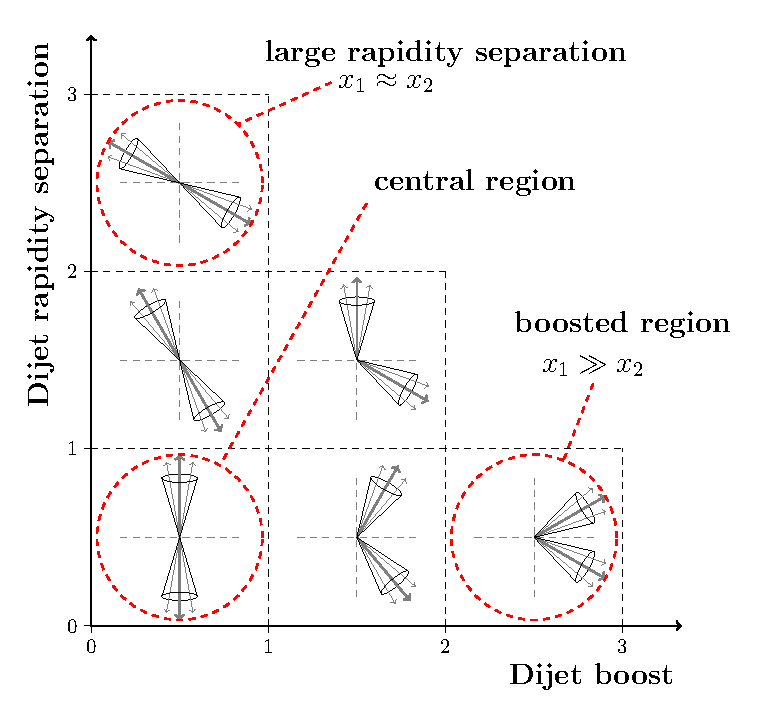
\includegraphics[width=0.6\textwidth]{figures/drawings/ybys_hint.pdf}
    \caption[Illustration of dijet topologies various \ystar and \yboost bins.]{
             An illustration of dijet event topologies as they are measured in
             the various \ystar and \yboost bins. Especially the separation of
             same-side and opposite-side dijet events allows to draw conclusions about
             the proton PDFs as different fractional proton momenta are accessed.}
    \label{fig:intro_ybys_hint}
\end{figure}

In Chapter~\ref{sec:theoretical_foundations}, the theoretical foundations for
dijet production at hadron colliders are outlined. An overview of the Standard
Model of particle physics with a focus on perturbative QCD is given.
Furthermore, the relativistic kinematics of dijet production is explained.
Chapter~\ref{sec:experimental_setup} summarizes the experimental setup of the
CMS detector and the measurement and reconstruction of jets. 

The theoretical considerations for the definition of the observables as well as
the accuracy of the NLO calculations are discussed in
Chapter~\ref{sec:theory_predictions}. The measurement of the triple-differential
dijet cross section with the CMS detector is presented in
Chapter~\ref{sec:measurement}. The measurement is scrutinized in a multitude
of studies of the detector and reconstruction efficiencies and a careful
determination of all uncertainties. Furthermore, the cross sections are
corrected for detector effects in an interative unfolding procedure and are
compared to pQCD calculations at NLO accuracy.

The thesis is round off with the PDF sensitivity studies presented in
Chapter~\ref{sec:pdf_constraints}, in which the constraints on the proton PDFs
are elaborated. Moreover, a simultaneous fit of the PDFs and the strong coupling
is performed to determine the coupling with best precision.

